% !TEX spellcheck = en_US

\documentclass[conference]{IEEEtran}
\usepackage{cite}
\usepackage{amsmath,amssymb,amsfonts}
\usepackage{algorithmic}
\usepackage{graphicx}
\usepackage{textcomp}
\usepackage{xcolor}
\usepackage{colortbl}
% add hyperlinks, delete all .aux files if adding hyperref after previous build
\usepackage{hyperref}
% support for unicode charcters like "é" and "ñ"
\usepackage[T1]{fontenc}
% Provides generic commands \degree, \celsius, \perthousand, \micro and \ohm
\usepackage{gensymb}
% splits a section into multiple columns
\usepackage{multicol}
\def\BibTeX{{\rm B\kern-.05em{\sc i\kern-.025em b}\kern-.08em
    T\kern-.1667em\lower.7ex\hbox{E}\kern-.125emX}}
\begin{document}

\title{Validation of Subhourly Clipping Loss Error Corrections}

\author{\IEEEauthorblockN{Abhishek Parikh\textsuperscript{1}, Kevin Anderson\textsuperscript{2}, Kirsten Perry\textsuperscript{2}, William B. Hobbs\textsuperscript{3}, Rounak Kharait\textsuperscript{1},}
\IEEEauthorblockN{and Mark A. Mikofski\textsuperscript{1}}
	\IEEEauthorblockA{\textsuperscript{1}DNV, San Diego, CA, 92123, USA }
    \IEEEauthorblockA{\textsuperscript{2}NREL, Golden, CO, 80401, USA }
    \IEEEauthorblockA{\textsuperscript{3}Southern Company, Birmingham, AL, 35203, USA }}

\maketitle

\begin{abstract}
Under-performance of solar PV systems is an important issue that increases risks for stakeholders, including developers, investors and operators. Recently some attention has focused on underestimation of inverter clipping losses as a possible source of over-prediction where sub-hourly solar variability is high. Several models and data sets have been analyzed over the past few years, with the aim of quantifying, predicting, and correcting underestimated clipping loss errors for sites with high DC/AC ratio and solar variability. In this report, we compare operational data with a machine learning model developed at NREL to correct energy assessments based on hourly weather. In addition, the model is expanded to include site-specific information such as DC/AC ratio and modeled PV power as factors, so that the model is flexible enough to be used for estimating clipping loss error in energy assessments for a wide variety of sites. 
\end{abstract}

\begin{IEEEkeywords}
inverter, clipping, solar, irradiance, variability, performance, modeling, TMY
\end{IEEEkeywords}

\section{Introduction}
In its report "2020 Solar Risk Assessment" \cite{Matsui2020}, kWh Analytics warned that systematic underproduction across the industry exposes investors to increased risk. DNV found that a sample of 39 projects from 2019 were under-performing compared to their pre-construction energy assessments by up to 3\% on average, as shown in Fig.~\ref{fig:project-underperformance}. NextEra estimates that sub-hourly solar resource variability can affect actual energy production by approximately 1-4\%. Cormode, \textit{et al.}, explained that energy assessments based on hourly weather, like typical meteorological year (TMY) data sets, underestimate inverter clipping losses by up to 5\% for projects with intra-hourly solar variability, especially for high DC/AC ratios \cite{Cormode2019}. This is demonstrated in Fig.~\ref{fig:irradiance-and-power}, which shows irradiance and power output at 1-minute and 1-hour resolution in the top and bottom panels, respectively. On July 10th, there is little intra-hour variability, indicative of a mostly clear day where hourly and sub-hourly simulations are in close agreement. In contrast, July 13th has much higher solar variability, but no clipping is observed in the 1-hour output. However, the 1-minute resolution shows intermittent clipping all day long, indicating that not all of the available irradiance is used by the system, and the hourly simulations underestimate inverter clipping \cite{Kharait}.

% what does the team think about citing (non-peer-reviewed) PVPMC posters? one or more of the posters that Jon Allen has presented (with me, sometimes EPRI) could be worth citing. 

\begin{figure}[htbp]
\centerline{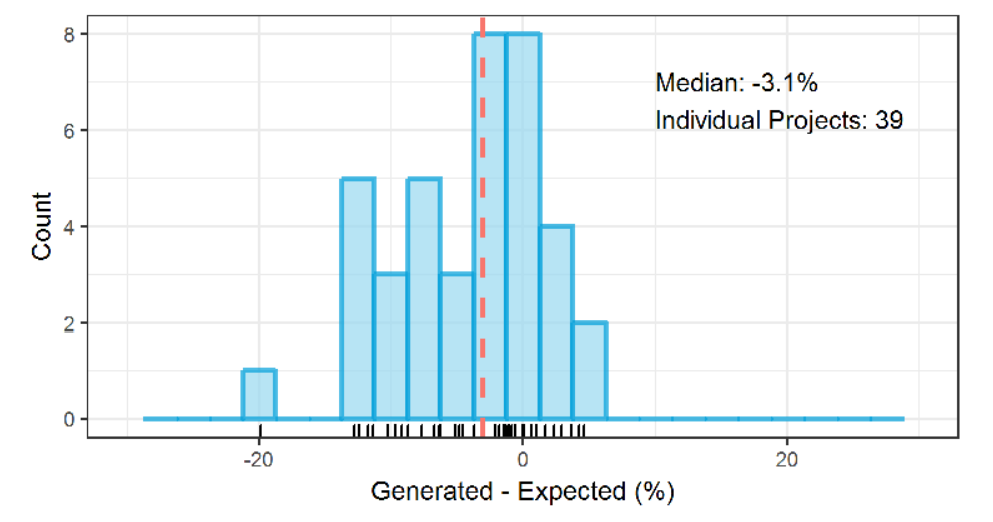
\includegraphics[width=9cm]{fig1.png}}
\caption{Project-average validation results for solar energy assessments. Each project-year was adjusted for interannual variability by scaling production by the ratio of TGY to historical monthly insolation.}
\label{fig:project-underperformance}
\end{figure}


\begin{figure}[htbp]
% combining the 1- and 60-min data on the same plot might be helpful. Additionally, using a second Y axis or normalizing GHI to 1000 w/m^2 and power to dc nameplate might help.
\centerline{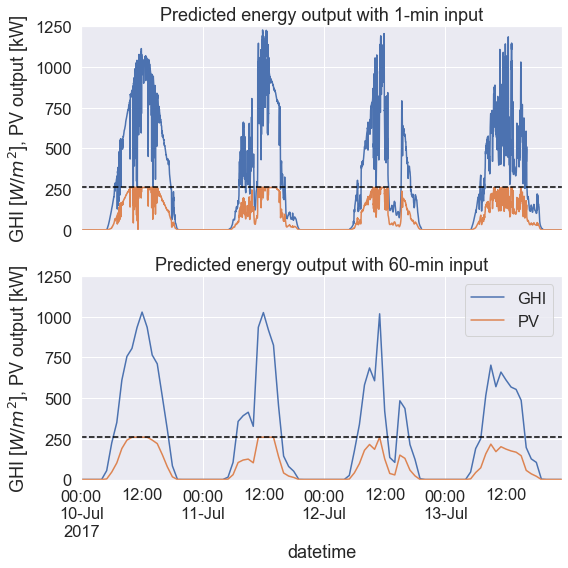
\includegraphics[width=9cm]{hourly_v_1-min_clipping.png}}
\caption{Irradiance input from the NIST test-bed weather station in Gaithersburg, MD, and predicted energy output using SolarFarmer at time-resolution of 1-minute, \textit{top panel}, and 1-hour, \textit{bottom panel}. The black dashed line in both panels shows the inverter-rated power, 260-kW.}
\label{fig:irradiance-and-power}
\end{figure}


Several methods have been proposed to correct clipping loss error in hourly predictions \cite{Cormode2019,Kharait,Anderson2020,Bradford}, but only NextEra validated their method with operational data \cite{Bradford}. 
% consider adding a reference to Hofmann 2014 (https://doi.org/10.1155/2014/808509), used in PV*SOL (see Lindemann presentation from 2017 PVPMC in ABQ, https://pvpmc.sandia.gov/resources-and-events/events/2017-8th-pv-performance-modeling-workshop/)
In this report, we adapt the NREL machine learning-based model \cite{Anderson2020} to predict clipping loss corrections and apply these corrections to hourly energy assessments. The adjusted energy assessment is then validated against operational data from the same site, and we report on the average and distribution of validation errors.  We have obtained data from two operating PV systems in Georgia, US and with a range of DC/AC ratios. In this paper, we will outline our method and present model validation results for these two systems. 

\section{Methods}

\subsection{Model}

The machine learning (ML) model developed at NREL has already been described in detail \cite{Anderson2020}. This model was adapted for the purpose of this research. A black-box XGBoost model was generated, with satellite data inputs, as well as features derived from these fields. In an extension of the model described in \cite{Anderson2020}, system DC/AC ratio and AC power outputs from the associated SAM model were added as continuous variable features. Specific model input parameters included the following:
\begin{itemize}
\item Min-max normalized POA, GHI, clearsky POA, clearsky GHI, and cell temperature
\item First-order differenced normalized POA
\item Difference between Clearsky POA and POA
\item System DC/AC ratio
\item Modeled AC power (taken from the SAM simulation) 
\end{itemize}
The model was trained using high quality irradiance measurements from SURFRAD \cite{Augustine2000} and 1-minute to 30-minute clipping loss errors predicted using SAM \cite{Freeman2018}. The resulting trained model was then used to make predictions at the operational sites.

\subsection{Sites}

For the validation, two operational sites in Georgia were chosen. The system parameters of the two solar sites used for validation are provided in Table~\ref{table1}. These sites were selected for their high DC/AC ratio, and 1-minute data sampling frequency.

\begin{table}[htbp]
\caption{System Parameters}
\begin{center}
\begin{tabular}{ |c|c|c| } 
\hline
& Site A & Site B \\
\hline
Array type & Tracking & Tracking \\
\hline
Array azimuth & 180$^{\circ}$ & 180$^{\circ}$\\
\hline
DC capacity & 27 MW & 43 MW\\
\hline
AC capacity & 19 MW & 30 MW \\
\hline
DC/AC Ratio & 1.42 & 1.43 \\
\hline
Ground coverage ratio & 0.3 & 0.3 \\
\hline
\end{tabular}
\end{center}
\label{table1}
\end{table}



\subsection{Validation}
A challenge in validating the clipping loss correction model is the lack of quality high-frequency irradiance measurements that are co-located with operational PV systems. Therefore this model differs from traditional approaches for model training and validation because it relies on SURFRAD measurements and SAM-simulated data to train the model, but uses operational data from different sites for validation. So no holdout methods are required in validating this model because the training and validation data sets are already independent. The downside of this method is that any systematic biases in SAM are introduced into the clipping loss correction model. In future work, if a large population of high-frequency irradiance and co-located operational data are obtained, the model can be retrained holding out a subset of the data for validation. This procedure would have the benefit of incorporating any physical effects that are not captured by SAM.

Quality of operational datasets is vital to avoid disruption of validation. Data points in the operational dataset related to plant sub-performance instances are considered to be outliers from the validation's standpoint and need to be removed. However, detecting sub-performance from inverter output is challenging. For this validation effort, the bias change is presented for both unfiltered and filtered data points. For filtering, data points that met the following criteria were removed: 
\begin{itemize}
\item The difference between the measured, on-site POA and the modeled POA calculated using the PSM data is less than 5\% 
\item The difference between actual power and simulated power of a particular timestep is more than 25\%. 
\end{itemize}
For site A and site B, 60.5\% and 55.1\% of the data is retained after applying the data filter, respectively.

In addition, high clipping errors occur during periods where the plant observes DC clipping (usually corresponding to higher irradiance), and high fluctuations in the irradiance. For the purpose of this validation, the fluctuations are quantified by calculating the variability index based on \cite{Stein}. The variability index is normally defined on GHI. However, since only on-site measured POA was available, the variability index for this study was calculated and aggregated at 30-min intervals using the on-site POA measured at a 1-min frequency. Since the ML model should be correcting only those periods with such conditions, the change is split into sets of low and high variability index. Periods are divided into three sets based on their variability index value:
\begin{itemize}
\item Low variability index  $(\leq10)$ 
\item Medium variability index  $(>10$ \& $\leq50)$. 
\item High variability index $(>50)$
\end{itemize}
Table.~\ref{var_index_breakdown} shows the composition of the on-site data based on the variability index. For this validation, two complete years of operational data from site A are used, and one complete year of operational data from site B is used.
% is this 50% of plant nameplate, or 50% of one of the power values for the individual timestep? 
% it would be good to note the # or % of intervals that were excluded


\begin{table}[htbp]
\caption{Composition of data based on variability index}
\begin{center}
\begin{tabular}{ |c|c|c| } 
\hline
& Site A & Site B \\
\hline
Low variability index $(\leq10)$ & 62\% & 63\% \\
\hline
Medium variability index $(>10$ \& $\leq50)$ & 21\% & 20\% \\
\hline
High variability index $(>50)$ & 17\% & 17\% \\
\hline
\end{tabular}
\end{center}
\label{var_index_breakdown}
\end{table}


The bias in model results is used to measure the reduction in clipping loss errors from the hourly energy assessment, and to identify if there are any unknown factors that are systematically affecting the results. Bias and mean bias error (MBE), the two metrics used to evaluate model performance in this study, are described in detail below.

\begin{itemize}
\item \textbf{Bias}: Delta between the corrected energy assessment predictions and the measured operational data. Positive bias means over-predicted energy output:
\begin{equation}
\Delta E={E_\text{predicted}} - {E_\text{measured}}\label{eq:bias}
\end{equation}
where $E$ is the energy output.
\item \textbf{Mean bias error (MBE)}: Average of the bias. Please note that a low MBE might hide seasonal or diurnal bias:
\begin{equation}
\mathit{MBE}=\frac{\sum_{n=1}^N{\Delta_n}}{N}\label{eq:mbe}
\end{equation}
Where $n$ is a single timestep, and $N$ is the total period of time. 
\end{itemize}


\section{Results}

30-minute NSRDB data from each site was fed into the ML model to make clipping error predictions. Model input parameters are previously described in the Methods section.

Time steps with a higher variability index should have higher clipping errors. Our results, shown in Figure ~\ref{fig:DCS-vi-clec-heatmap}, support this statement. Fig.~\ref{fig:DCS-vi-clec-heatmap} displays a heat map of average variability index, as well as the average clipping loss error correction predicted for site A. Generally, higher variability periods coincide with higher clipping loss corrections, usually occurring in the middle of the day around 1 pm, and during summer months.

\begin{figure}[htbp]
\centerline{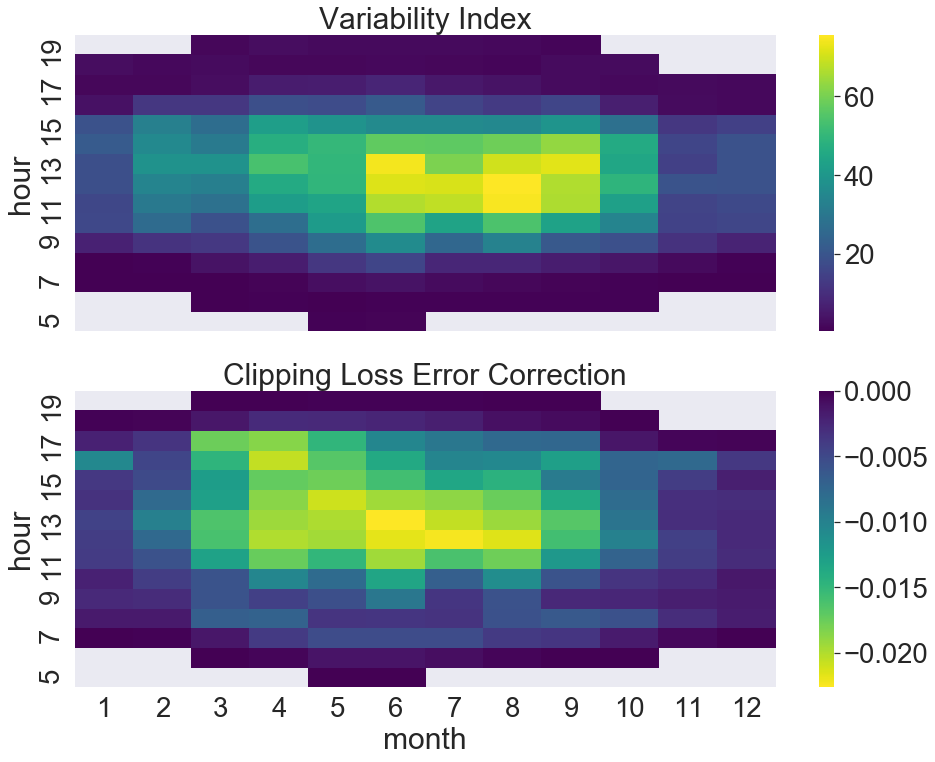
\includegraphics[width=9cm]{DCS_VI_CLEC_heatmap.png}}
\caption{The first sub-figure shows the average variability index calculated at site A. The variability index is calculated and aggregated at a 30-min interval using on-site POA measured at a 1-min time resolution. In the second sub-figure, the average clipping error correction calculated for site A using the ML model is shown. The model predicts the clipping error correction factor for each 30-min interval.}
\label{fig:DCS-vi-clec-heatmap}
\end{figure}

Fig.~\ref{fig:DCS-inv-modelbias-poa-scatter} shows the actual power of an inverter against the actual POA. At a higher variability index, the power is lower and corresponds to higher model bias.

\begin{figure}[htbp]
\centerline{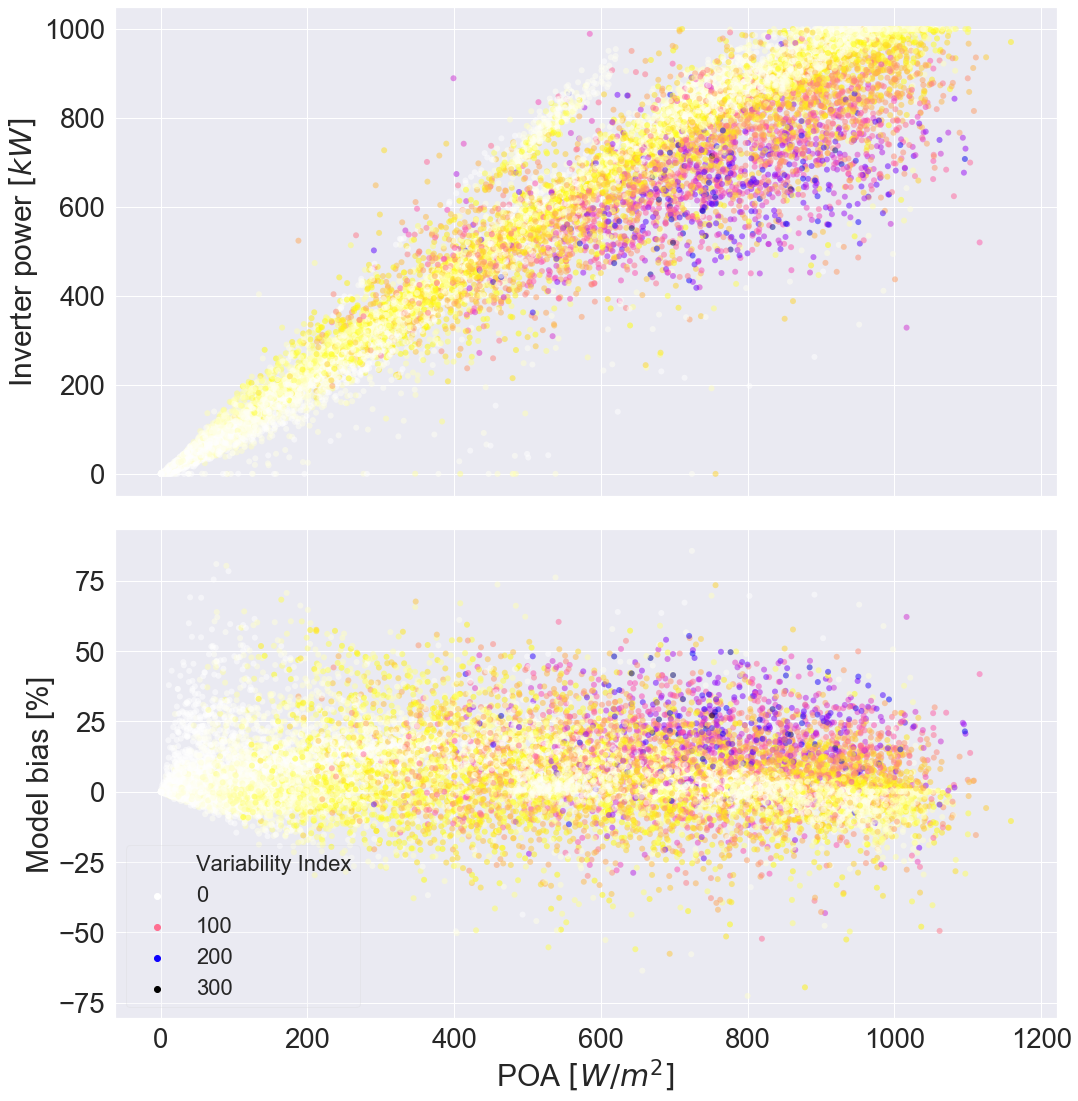
\includegraphics[width=9cm]{DCS_Inv_ModelBias_POA_with_VI.png}}
\caption{Inverter power and bias in modeled power for a 1000 kW rated inverter at site A. Lower power and higher model bias are observed at a higher variability index.}
\label{fig:DCS-inv-modelbias-poa-scatter}
\end{figure}

For the energy model, 30-minute NSRDB data was used to generate a time series of energy estimates for site A and site B. Then, these energy estimates were corrected using the clipping loss error corrections predicted by the ML model. As observed, the overall shift in the bias is small for each time series. Table.~\ref{table2} summarize the mean bias errors in the energy models before and after applying the correction, for sites A and B respectively. As indicated by Fig.~\ref{fig:DCS-vi-clec-heatmap} and Fig.~\ref{fig:DCS-inv-modelbias-poa-scatter}, the magnitude of the clipping loss error correction should be high during time steps with a high variability index and low during time steps with a low variability index. Hence, the bias is explored based on the low, medium and high variability index categories described in the Validation section. Part (A) of Fig.~\ref{fig:DCS-modelbias-cdf} and Fig.~\ref{fig:PAW-modelbias-cdf} show the cumulative distribution of the overall bias before and after correction. Part (B) of these figures break the bias based on the variability index. The breakdown shows that the change in bias is high for the points with high variability index whereas it is small for the points with low variability index. This observation corroborates the relation between variability index and clipping loss error corrections discussed above.

\begin{table}[htbp]
\caption{Results summary by Site}
\begin{center}
\scalebox{0.96}{%
\begin{tabular}{|c|c|c|c|c| } 
\hline
Site & Metric & Before     & After      & Change\\
     &        & correction & correction & [\%]\\
\hline
Site A & Overall MBE & 5.4\% & 4.8\% & -0.6\\
\hline
Site A & MBE (High VI) & 10.7\% & 9.3\% & -1.4\\
\hline
Site A & MBE (Medium VI) & 4.3\% & 3.5\% & -0.8 \\
\hline
Site A & MBE (Low VI) & 4.4\% & 4.0\% & -0.4\\
\hline
Site B & Overall MBE & 7.8\% & 6.7\% & -1.1\\
\hline
Site B & MBE (High VI) & 10.4\% & 7.9\% & -2.5\\
\hline
Site B & MBE (Medium VI) & 7.7\% & 6.3\% & -1.4\\
\hline
Site B & MBE (Low VI) & 7.1\% & 6.5\% & -0.6\\
\hline
\end{tabular}}
\end{center}
\label{table2}
\end{table}



%\begin{table}[htbp]
%\caption{Results summary for Site A}
%\begin{center}
%\begin{tabular}{ |c|c|c|c| } 
%\hline
%Metric & Before correction & After correction & \% Change\\
%\hline
%Overall MBE & 5.4\% & 4.8\% & %-0.6\\
%\hline
%MBE (High VI) & 10.7\% & 9.3\% & -1.4\\
%\hline
%MBE (Medium VI) & 4.3\% & 3.5\% & -0.8 \\
%\hline
%MBE (Low VI) & 4.4\% & 4.0\% & %-0.4\\
%\hline
%\end{tabular}
%\end{center}
%\label{table2}
%\end{table}


\begin{figure}[htbp]
\centerline{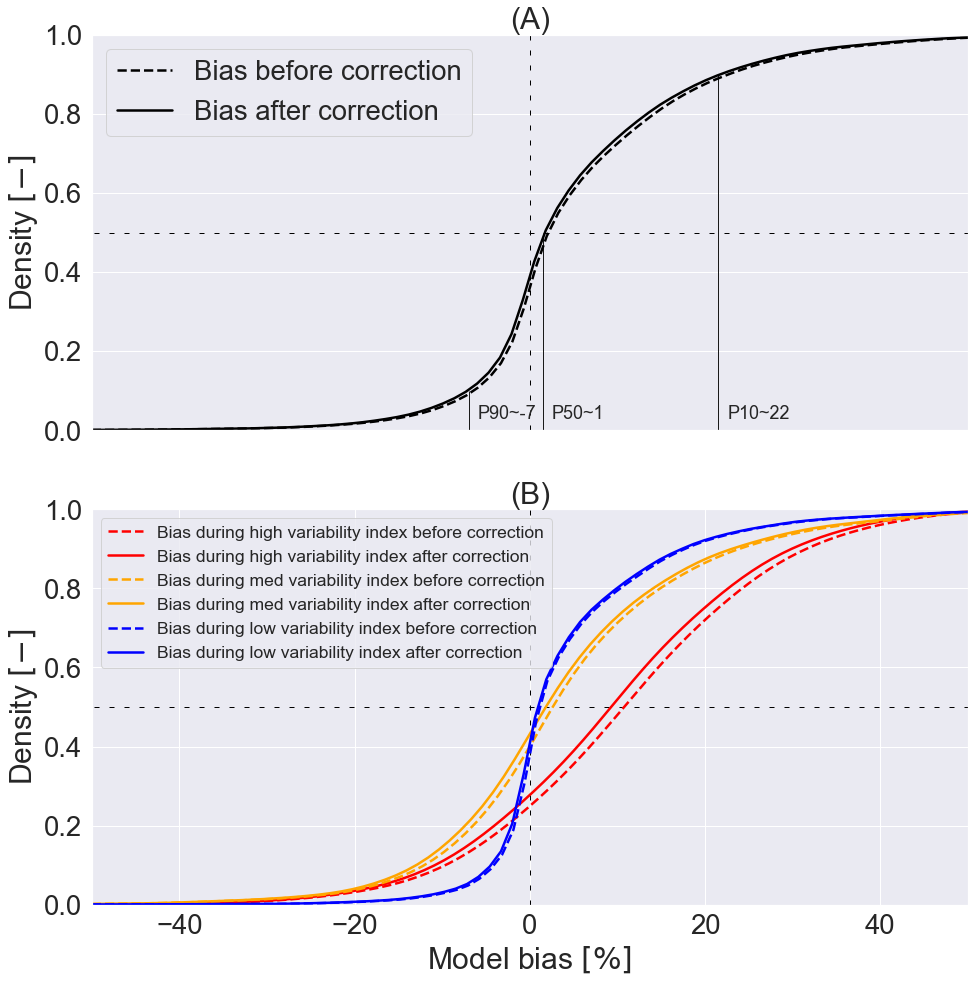
\includegraphics[width=9cm]{DCS_ModelBias_breakdown_CDF_v4.png}}
\caption{CDF of Model bias for site A before data filtering}
\label{fig:DCS-modelbias-cdf}
\end{figure}


%\begin{table}[htbp]
%\caption{Results summary for Site B}
%\begin{center}
%\begin{tabular}{ |c|c|c|c| } 
%\hline
%Metric & Before correction & After correction & \% Change\\
%\hline
%Overall MBE & 7.8\% & 6.7\% & -1.1\\
%\hline
%MBE (High VI) & 10.4\% & 7.9\% & -2.5\\
%\hline
%MBE (Medium VI) & 7.7\% & 6.3\% & -1.4\\
%\hline
%MBE (Low VI) & 7.1\% & 6.5\% & -0.6\\
%\hline
%\end{tabular}
%\end{center}
%\label{table3}
%\end{table}

\begin{figure}[htbp]
\centerline{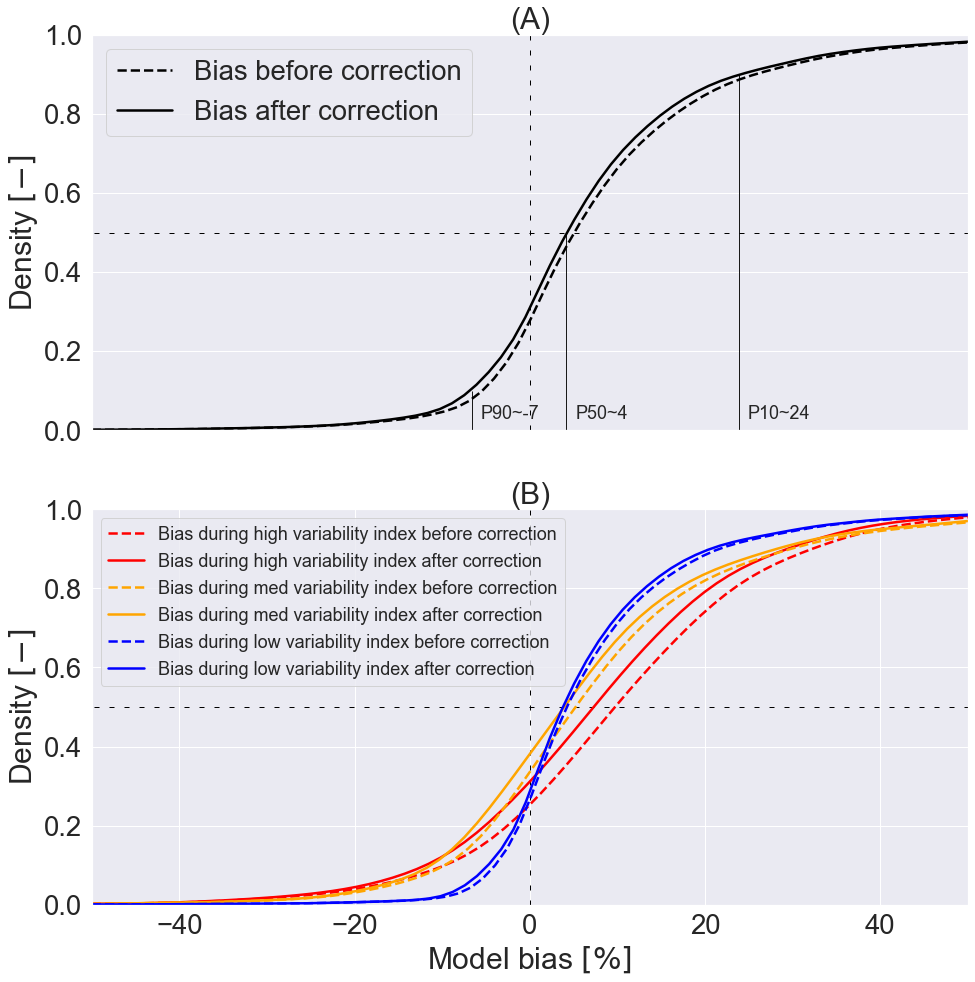
\includegraphics[width=9cm]{PAW_ModelBias_breakdown_CDF_v4.png}}
\caption{CDF of Model bias for site B before data filtering}
\label{fig:PAW-modelbias-cdf}
\end{figure}

The overall model bias in Fig.~\ref{fig:DCS-modelbias-cdf} and Fig.~\ref{fig:PAW-modelbias-cdf} can be attributed to many reasons. Factors like the difference in the resource measured on-site and NSRDB dataset, site specific sub-performance, incorrect loss assumption in the energy model, etc impact the bias along with the clipping loss errors. However, for a given data point, it is unrealistic to have a bias of greater than 25\% in power when the bias in POA is less than 5\%. Consequently, points fitting this logic are removed and the bias change is recalculated. Table.~\ref{results_after_filter} summarize the mean bias errors in the filtered data points of the energy models before and after applying the correction, for sites A and B respectively. Fig.~\ref{fig:DCS-modelbias-after-filter-cdf} and Fig.~\ref{fig:PAW-modelbias-after-filter-cdf} show the bias before and after the correction for this filtered dataset. Compared to the CDFs plotted for the unfiltered dataset, these plots show a much tighter distribution as the outliers are removed. 

\begin{table}[htbp]
\caption{Results summary by Site, after filtering}
\begin{center}
\scalebox{0.96}{%
\begin{tabular}{ |c|c|c|c|c| } 
\hline
Site & Metric & Before     & After      & Change\\
     &        & Correction & Correction & [\%]\\
\hline
Site A & Overall MBE & 2.3\% & 1.8\% & -0.5\\
\hline
Site A & MBE (High VI) & 10.6\% & 9.2\% & -1.4 \\
\hline
Site A & MBE (Medium VI) & 3.1\% & 2.4\% & -0.7\\
\hline
Site A & MBE (Low VI) & 1.1\% & 0.8\% & -0.3\\
\hline
Site B & Overall MBE & 3.6\% & 2.8\% & -0.8\\
\hline
Site B & MBE (High VI) & 8.7\% & 6.1\% & -2.6\\
\hline
Site B & MBE (Medium VI) & 4.4\% & 3.0\% & -1.4\\
\hline
Site B & MBE (Low VI) & 2.8\% & 2.4\% & -0.4\\
\hline
\end{tabular}}
\end{center}
\label{results_after_filter}
\end{table}


\begin{figure}[htbp]
\centerline{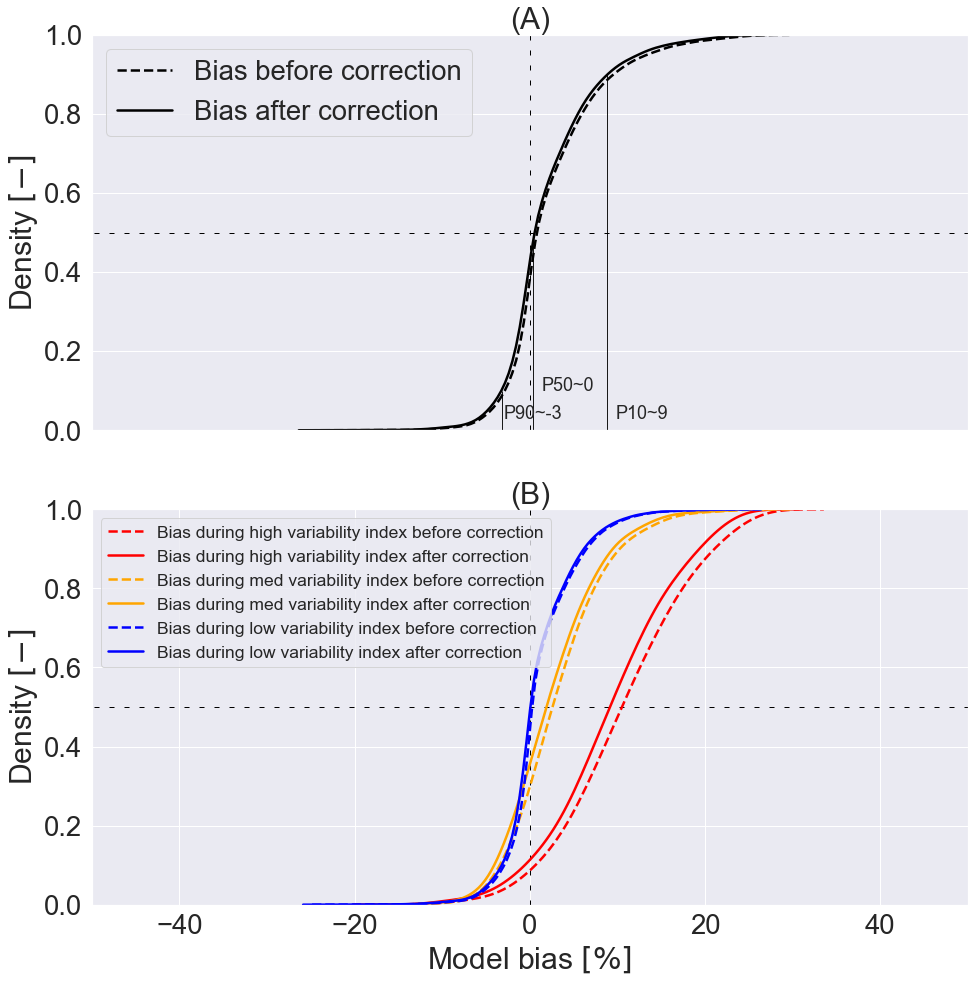
\includegraphics[width=9cm]{DCS_ModelBias_breakdown_AFTER_filter_CDF_v4.png}}
\caption{CDF of Model bias for site A after data filtering}
\label{fig:DCS-modelbias-after-filter-cdf}
\end{figure}

\begin{figure}[htbp]
\centerline{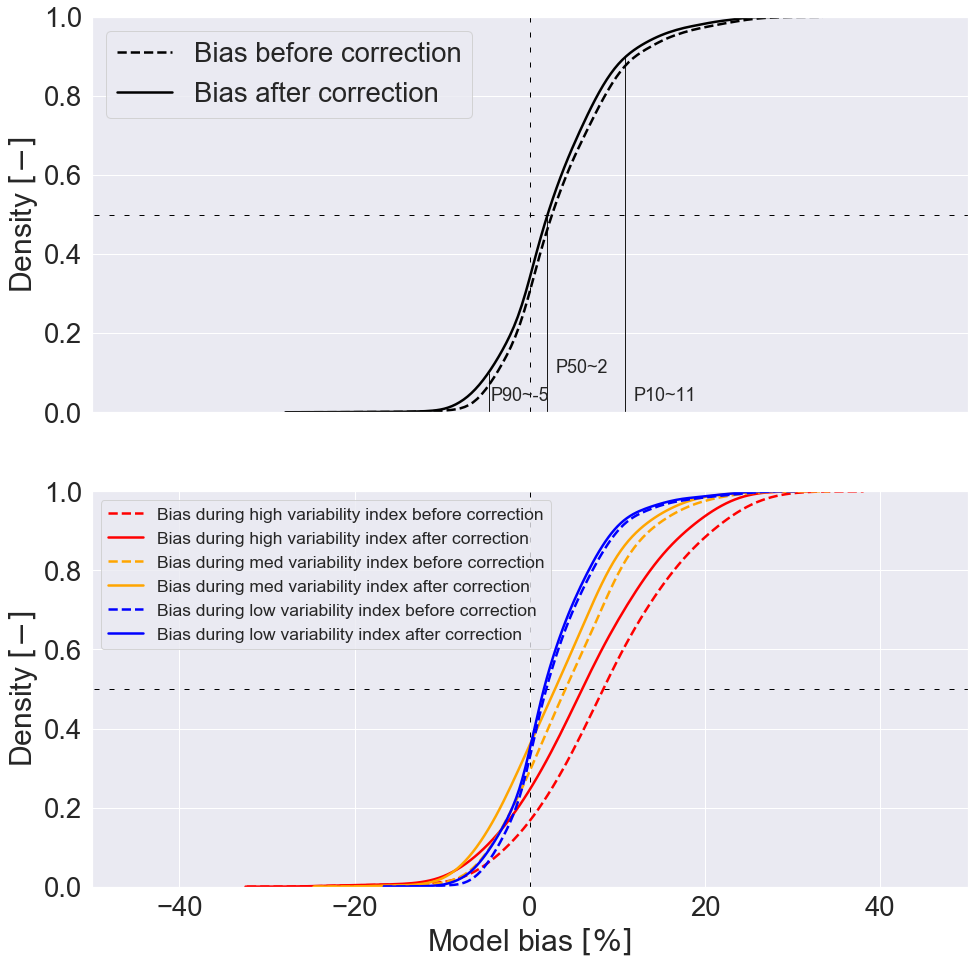
\includegraphics[width=9cm]{PAW_ModelBias_breakdown_AFTER_filter_CDF_v4.png}}
\caption{CDF of Model bias for site B after data filtering}
\label{fig:PAW-modelbias-after-filter-cdf}
\end{figure}

\section{Conclusions}
Over-prediction occurs in typical energy assessments that use hourly data if the sites have sub-hourly solar variability and high DC/AC because clipping losses are underestimated. These errors have been quantified using a machine-learning model trained on high-frequency solar irradiance data and simulated operational data to create clipping loss error corrections. The corrections were applied to a typical hourly energy assessment of an existing operational site and compared to the measured output from the same site. The bias before the correction can have multiple factors other than clipping loss errors. This model reduces the bias in the energy assessments by 0.5\% and 0.8\% done for site A and site B respectively.

\section*{Acknowledgment}

This work was authored in part by Alliance for Sustainable Energy, LLC, the manager and operator of the National Renewable Energy Laboratory for the U.S. Department of Energy (DOE) under Contract No. DE-AC36-08GO28308. Funding provided by the U.S. Department of Energy’s Office of Energy Efficiency and Renewable Energy (EERE) under Solar Energy Technologies Office (SETO) Agreement Numbers 34348. The views expressed in the article do not necessarily represent the views of the DOE or the U.S. Government. The U.S. Government retains and the publisher, by accepting the article for publication, acknowledges that the U.S. Government retains a nonexclusive, paid-up, irrevocable, worldwide license to publish or reproduce the published form of this work, or allow others to do so, for U.S. Government purposes.

\bibliographystyle{IEEEtran}
% argument is your BibTeX string definitions and bibliography database(s)
\bibliography{IEEEabrv,bibliography}

\end{document}
